\section{System}
\label{sec:sys}

\begin{figure}[t!]
\begin{center}
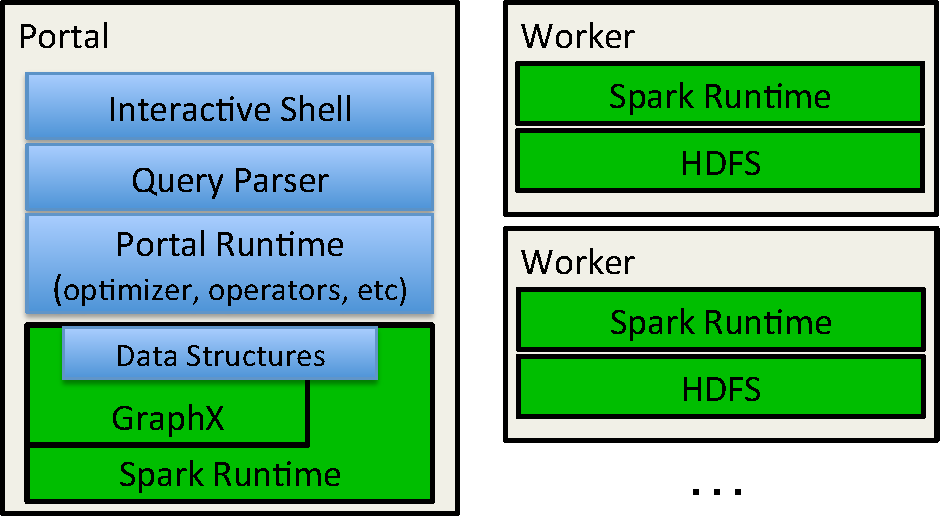
\includegraphics[height=1.4in]{figs/architecture.pdf}
\caption{\ql system architecture.}
\label{fig:arch}
\end{center}
\end{figure}

The \ql system builds on GraphX~\cite{DBLP:conf/osdi/GonzalezXDCFS14},
an Apache Spark library, as depicted in Figure~\ref{fig:arch}.  Green
boxes indicate built-in components, while blue are those we added for
\ql.  We selected Apache Spark because it is a popular open-source
system, and because of its in-memory processing approach.  All
language operators on \tgs are available through the public API of the
\ql library, and may be used like any other library in an Apache Spark
application.

%\subsection{Query Processing}
%\label{sec:queryp}

\eat{
\begin{figure}
\begin{center}
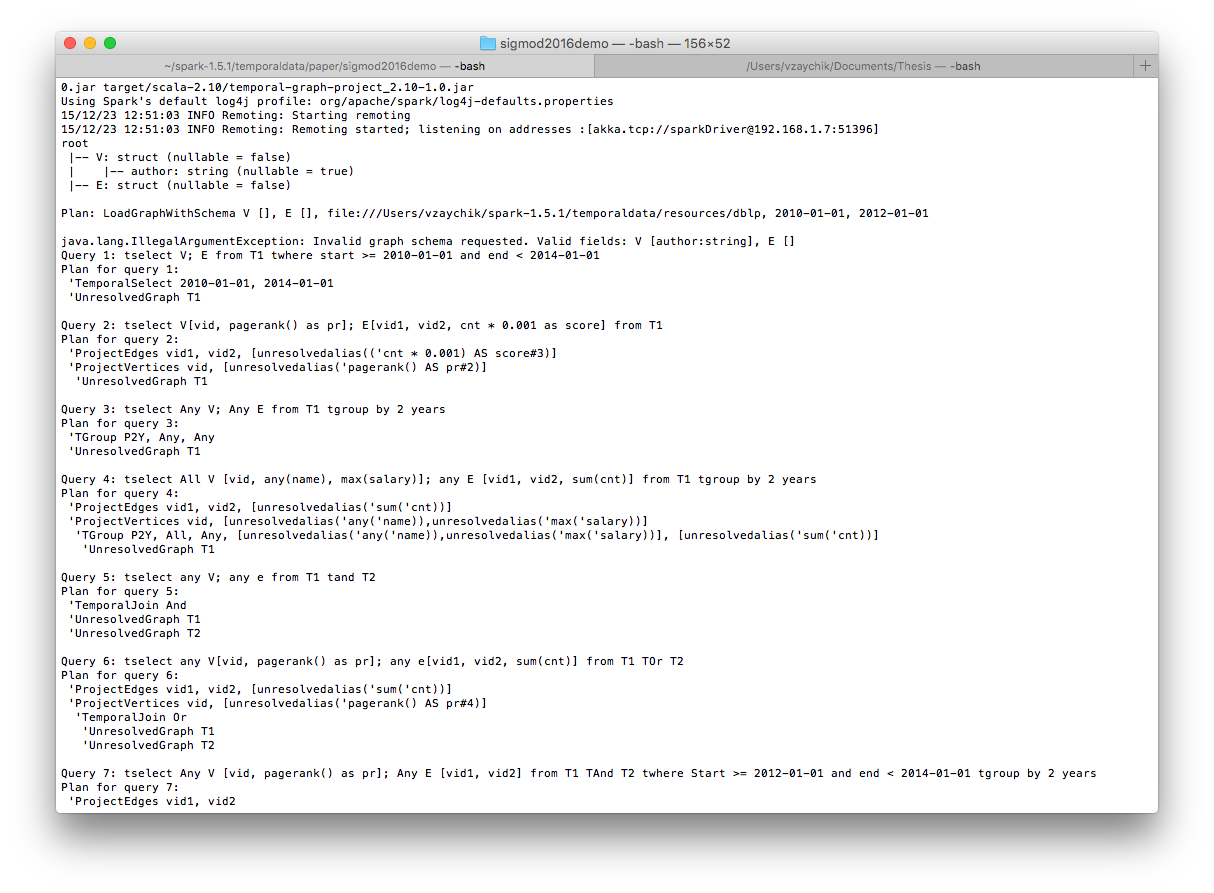
\includegraphics[width=3.2in]{figs/shell.png}
\caption{\ql shell session. PLACEHOLDER}
\label{fig:shell}
\end{center}
\end{figure}
}

{\bf Query evaluation.}  \ql query execution follows the traditional
query processing steps: parsing, logical plan generation and
verification, and physical plan generation.  \ql re-uses and extends
SparkSQL abstractions for these steps.  A \ql query is rewritten into
a sequence of operators, and some operators are reordered to improve
performance.  For example, pushing temporal aggregation before
temporal join can sometimes lead to more efficient performance.  A
temporal join query may be rewritten to include additional temporal
selection conditions, based on information about the temporal schema
of the \tgs being joined, which in turn significantly reduces data
load time.

We developed several different physical representations and
partitioning strategies that are selected at the physical plan
generation stage.  The \tgs are read from the distributed file system
HDFS and processed by Spark Workers, with the tasks assigned and
managed by the runtime.

{\bf Interactive shell.  Integration with SQL.} The \ql system
includes an interactive shell for exploratory data analysis.  Shell
users can define (materialized) \tg views, inspect query execution
plans and execute SQL queries with an embedded \ql view.  Consider
query \insql{Q3}, a SQL query that returns \insql{vid} and \insql{tr}
values of 20 vertices with the most significantly increasing
\insql{pagerank} trend.

\begin{enumerate}[leftmargin=*]
\item
 Define (materialized) views of \tg using standard SQL
  \insql{create view} command.
\item View optimized execution plans for defined views using
  \insql{describe} command.
\item View results of queries using SQL, with \ql queries either
  embedded in SQL, or a previously defined view.
\item View defined views and functions.
\end{enumerate}

%{\bf Integration with SQL.}  

\begin{small}
\begin{verbatim}
Q3:   Select   VF.vid, VF.tr  
      From     T5.toVerticesFlat() as VF
      Order by tr
      Limit    20
\end{verbatim}
\end{small}

An important part of \insql{Q3} is the use of
\insql{T5.toVerticesFlat()} in the \insql{From} clause.  This is an
operation provided by the \ql framework, which collects all vertices
in the union of snapshots of \insql{T5} into a single nested vertex
collection and flattens it into \insql{VF} (\underline{vid}:int,
\underline{start}:date, \underline{end}:date, tr:float, mx:float).
\insql{VF} can be used in SQL queries.  \ql also provides an operation
that returns a flattened collection of edges, called
\insql{toEdgesFlat()}.

\section{Graphical Query Composition}
\label{sec:gui}

\begin{figure}
\begin{center}
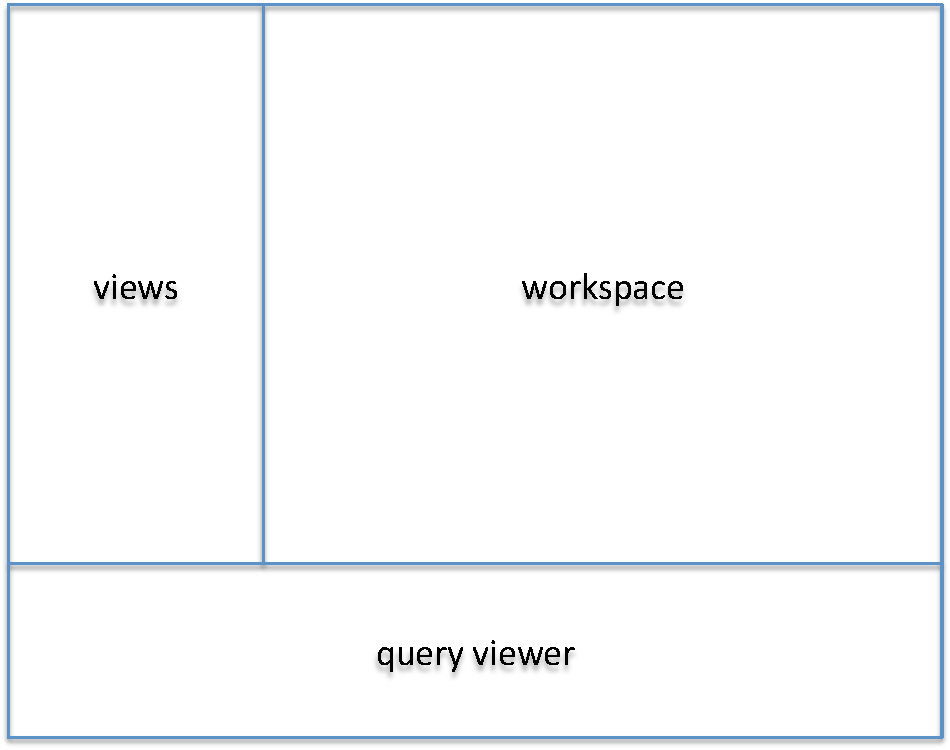
\includegraphics[width=3.2in]{figs/ui.pdf}
\caption{Graphical query composition. PLACEHOLDER}
\label{fig:ui}
\end{center}
\end{figure}

Evolving graph analysis is of interest to researchers in many domains,
as we already showed previously.  While \ql is declarative and, thus,
does not require computer science expertise to use, we want to reach a
wide audience.  For this reason, we are developing a graphical query
composition tool \qlui (Figure~\ref{fig:ui}).

\qlui users can compose queries by adding to and manipulating
\tg\\s in the workspace, where they are represented by their
timelines.  To temporally join two evolving graphs, for example, the
user can drag them to the workspace and place them close together.  If
the two graphs are not union-compatible, they will not snap together
and an error message is displayed to the user explaning the problem.
Union-compatibility is one of the more complex aspects of the
language, and it is our hope that a graphical representation of the
\tg temporal schema will reduce confusion.

To select a temporal subset of a \tg, the user can move the outside
border of the timeline.  To aggregate a \tg, the user can move the
border of any of the timeline periods and then specify the aggregation
functions through a drop-down menu.

As the query is composed graphically, its \ql representation is
updated in the Query view.  The user can also view the optimized
logical plan for the query in the Plan view.

